Die Monozelle, welche aus idealer Spannungsquelle und einem Widerstand besteht,
wird an ein Voltmeter angeschlossen. Das Voltmeter besitzt einen Widerstand von
\begin{equation*}
  R_{V}=10\cdot10^6\Omega.
\end{equation*}
So lässt sich die Leerlaufspannung der Monozelle bestimmen.
Nun wird ein regelbarer Widerstand R mit der Monozelle in Reihe geschaltet.
Mit einem ebenfalls in Reihe geschaltetem Amperemeter lässt sich eine Beziehung zwischen
Klemmenspannung $U_K$ und Strom I bestimmen. Es werden dazu mindestens 10 Wertepaare aufgenommen.
Im nächsten Versuchsteil wird einen entgegengerichtete Spannungsquelle hinter den Widerstand geschaltet.
Diese besitzt eine mindestens um 2V größere Spannung als die Monozelle, sodass der Strom auch in entgegengesetzter Richtung fließt.
Das Schaltbild ist in Abbildung \ref{fig:Gegenspannung} dargestellt.
Es werden wieder 10 Wertepaare von $U_K$ und I aufgenommen.
Für den letzten Teil des Experimentes wird die Gegenspannung wieder ausgebaut und die Monozelle durch einen RC-Generator ersetzt.
Dieser gibt eine Rechteckspannung aus. Hierzu werden wieder die Wertepaare $U_K$ und I bestimmt.
Für die Sinusspannung wird diese Messung wiederholt.

\begin{figure}[h!]
  \centering
  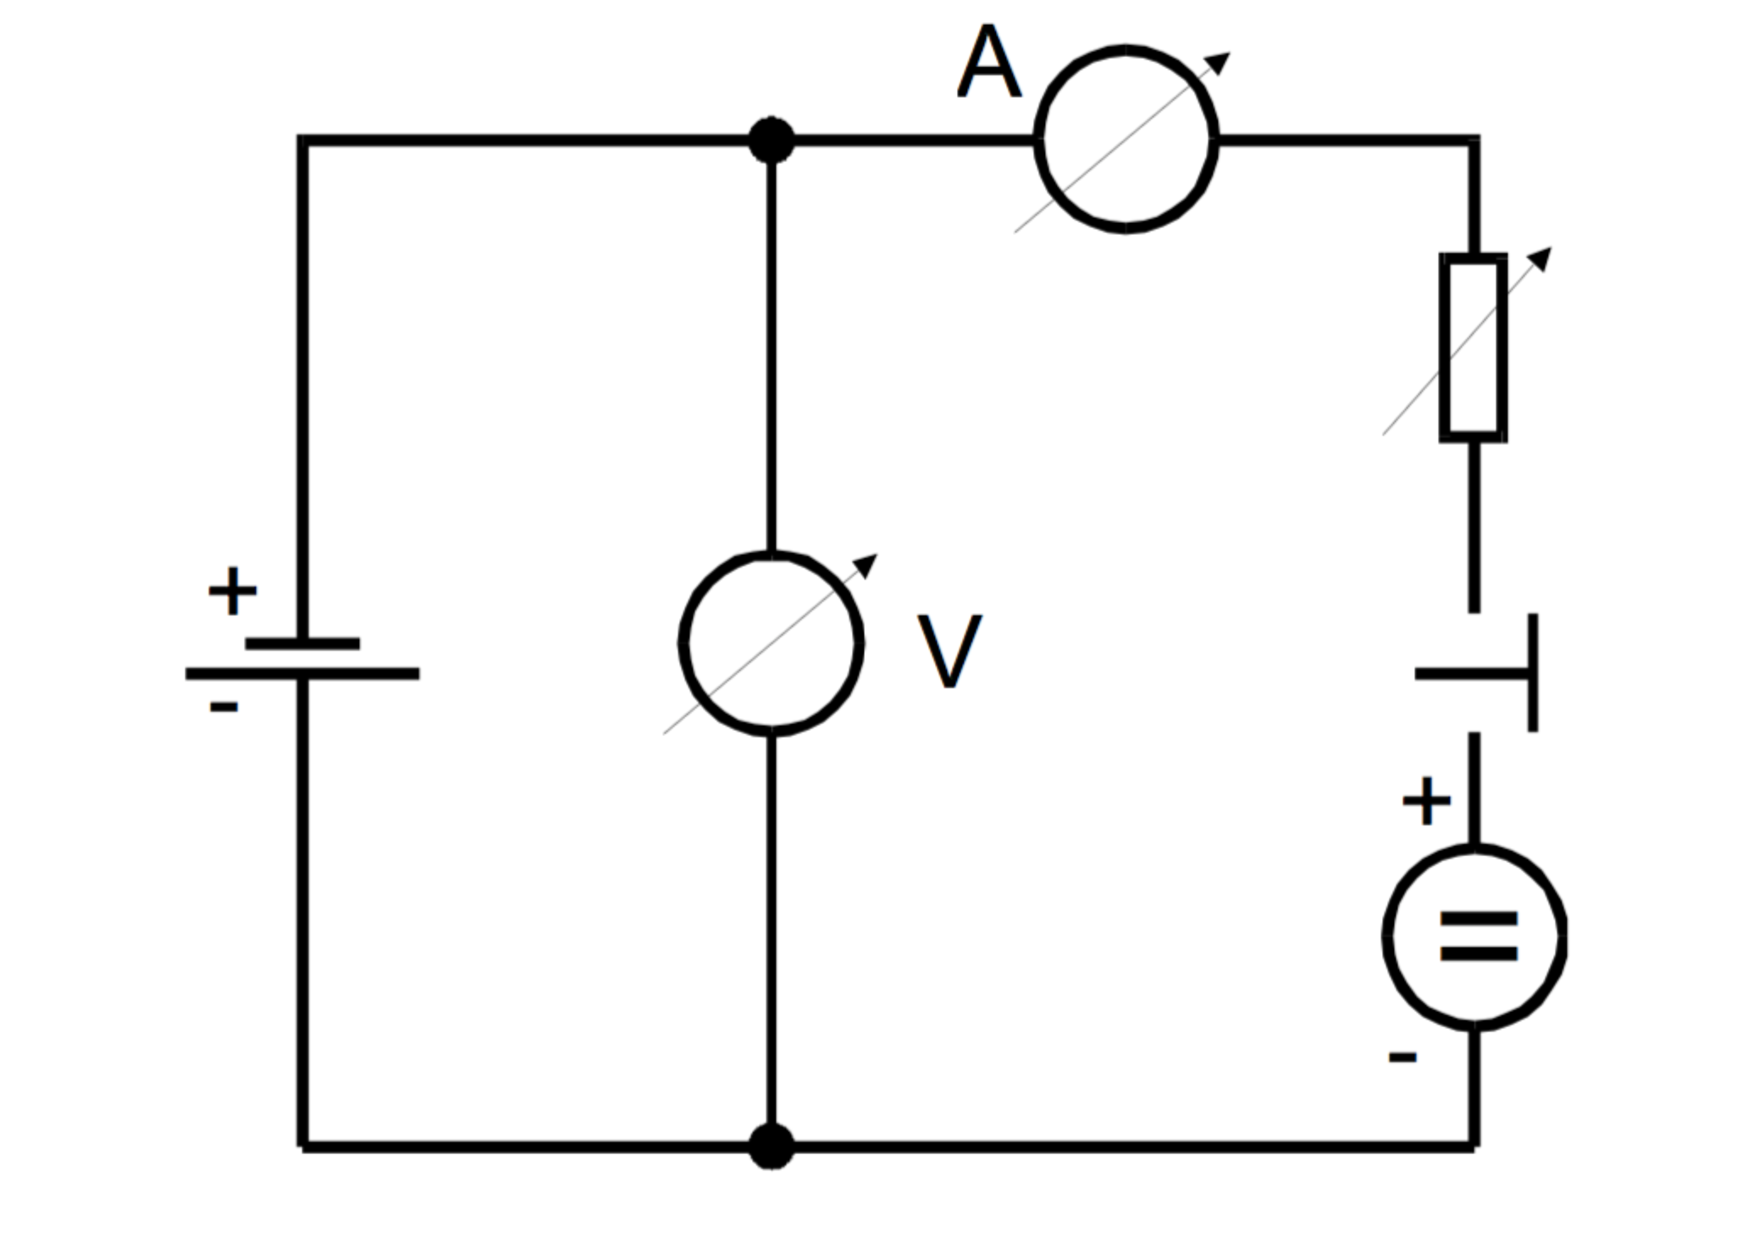
\includegraphics[width=0.7\textwidth]{Gegenspannung.pdf}
  \caption{Schaltbild mit Gegenspannung \cite{1}}
  \label{fig:Gegenspannung}
\end{figure}
